\section{Progettazione Logica}

In questa sezione viene illustrato il processo di “traduzione” dello schema concettuale in uno schema logico, con l’obiettivo di rappresentare i dati in modo preciso
ed efficiente. Il primo passo consiste nell’analizzare le eventuali ridondanze nel modello, al fine di ottimizzare la struttura complessiva. Successivamente, si procede
con l’eliminazione delle due generalizzazioni. Infine, viene presentato il diagramma
ristrutturato, con una descrizione delle modifiche apportate.

\subsection{Analisi Ridondanze}

L'attributo PACCHIATTIVI in CORRIERE esprime il numero di pacchi non ancora consegnati che sono associati a ogni corriere. Ciò corrisponde a una ridondanza dato che si tratta di un numero calcolabile contando, per ogni corriere, il numero di pacchi il cui corrispettivo TRACKING ha l'attributo STATUS diverso da \textit{"Consegnato"}.
Questo attributo viene modificato ogni volta che un pacco viene consegnato o associato al corriere. Viene invece visualizzato ogni mezz'ora per monitorare l'operato di ogni corriere. Il numero di pacchi associati al giorno per un corriere è in media di 120\footnote{\href{https://www.dire.it/26-02-2019/301816-video-a-milano-la-rabbia-dei-corrieri-di-amazon-quattro-minuti-a-consegna-troppo-pochi/}{Fonte di riferimento per i "120 pacchi al giorno". 2019}}.\\
Questo si riassume nelle due seguenti operazioni:
\begin{itemize}
    \item \textbf{Operazione 1 (120 volte al giorno)}: memorizza il numero di pacchi non consegnati associati ad ogni corriere.
    \item \textbf{Operazione 2 (48 volte al giorno)}: visualizza il numero di pacchi non consegnati associati ad ogni corriere
\end{itemize}


\begin{table}[H]
    \centering
    \begin{tabular}{p{2.5cm} p{4cm} p{5cm} p{3cm}}
    \toprule
    \textbf{Entità} & \textbf{Descrizione} & \textbf{Attributi} & \textbf{Identificatore} \\
    \midrule
    Filiale         & Filiale di un'azienda di spedizione & Nome, Città, Tipo, Indirizzo & Nome, Città \\
    
    Tracking        & Storico del Tracking di un pacco & DataOra, IdPacco, Status, Note, NomeCheckPoint, CittàCheckPoint & IdPacco, DataOra \\
    
    Pacco           & Elemento spedito & Id, Tipologia, Dimensioni, Costo, DataOrdine, DataSpedizione & Id \\
    
    Pacchi Assicurati & Pacco Assicurato & TipoAssicurazione & — \\
    
    Pacchi Regalo   & Pacco Regalo & Dedica, TipoCarta & — \\
    
    Cliente         & Proprietario del Pacco & Email, Nome, Cognome, Indirizzo, Telefono & Email \\
    
    Corriere        & Addetto alla spedizione di un pacco & C.F., Grado, Disponibilità, PacchiAttivi & C.F. \\
    \bottomrule
    \end{tabular}
    \caption{Tabella delle Entità}
    \label{tab:entità}
\end{table}

\begin{table}[H]
    \centering
    \begin{tabular}{clcc}
    \toprule
    \textbf{Relazione} & \textbf{Descrizione} & \textbf{Componente} & \textbf{Attributi}  \\ [0.5ex] 
    \midrule
        Sede & Sede di un Corriere & Corriere, Filiale & Attuale\\
        Transito & Posizione Pacco & Tracking, Filiale & \\
        Status & Informazioni sul tracciamento del pacco & Pacco, Tracking & \\
        Contiene & Composizione dei Bundle & Pacco,Bundle & Quantità \\
        Ordine & Ordine di un pacco di un cliente & Cliente, Pacco &  \\
        Consegna & Consegna di un pacco da parte di un Corriere & Corriere, Pacco & \\
        \bottomrule
    \end{tabular}
    \caption{Tabella delle Relazioni}
    \label{tab:relzioni}
\end{table}



Assumendo i seguenti volumi nella base di dati:

\begin{table}[H]
\centering
\begin{tabular}{lcc}
\toprule
\textbf{Concetto} & \textbf{Costrutto} & \textbf{Volume} \\ [0.5ex]
\midrule
    Corriere & E & 1000 \\
    Tracking & E & 120 000 \\
    Pacco & E & 120 000 \\
    Consegna & R & 120 000 \\
    Status & R & 120 000 \\
\bottomrule
    \end{tabular}
    \caption{Tabella dei Volume}
\end{table}


la seguente analisi serve per stabilire se sia utile o meno tenere l’attributo ridondante
PACCHIATTIVI in CORRIERE.

\textbf{Con Ridondanza:} Analizziamo prima il costo totale con ridondanza.\\
\textbf{Operazione 1:} 

\begin{table}[H]
\centering
\begin{tabular} {lllll}
    \toprule
    \textbf{Concetto} & \textbf{Costrutto} & \textbf{Accessi} & \textbf{Tipo} & \textbf{Accessi al giorno}\\ [0.5ex]
    \midrule
        Tracking & E & 1 & S & 120\\
        Pacco & E & 1 & S & 120\\
        Status & R & 1 & S & 120\\
        Corriere & E & 1 & S & 120\\
    \bottomrule
\end{tabular}
\caption{Tabella dei Volume}
\end{table}


\textbf{Operazione 2:}\\
\begin{table}[H]
\centering
\begin{tabular} {lllll}
    \toprule
    \textbf{Concetto} & \textbf{Costrutto} & \textbf{Accessi} & \textbf{Tipo} & \textbf{Accessi al giorno}\\ [0.5ex]
    \midrule
        Corriere & E & 1 & L & 48\\
    \bottomrule
\end{tabular}
\caption{Tabella dei Volume}
\end{table}

Assumendo costo doppio per gli accessi in scrittura rispetto a quelli in lettura, il costo totale con ridondanza è:
Costo totale con ridondanza = 120*4*2+48*1= 1080+48=1128

\textbf{Senza Ridondanza:} Analizziamo prima il costo totale senza ridondanza.
\begin{itemize}
    \item \textbf{Operazione 1:} 
     
        \begin{table}[H]
        \centering
        \begin{tabular} {lllll}
        \toprule
        \textbf{Concetto} & \textbf{Costrutto} & \textbf{Accessi} & \textbf{Tipo} & \textbf{Accessi al giorno}\\ [0.5ex]
        \midrule
            Tracking & E & 1 & S & 120\\
            Pacco & E & 1 & S & 120\\
            Status & R & 1 & S & 120\\ 
        \bottomrule
           \end{tabular}
            \caption{Tabella dei Volume}
    \end{table}

    \item \textbf{Operazione 2(Con circa 120 000/1000=120 pacchi consegnati al giorno):}
        \begin{table}[ht]
        \centering
        \begin{tabular} {lcccc}
        \toprule
        \textbf{Concetto} & \textbf{Costrutto} & \textbf{Accessi} & \textbf{Tipo} & \textbf{Accessi al giorno}\\ [0.5ex]
        \midrule
            Corriere & E & 1 & L & x48\\
            Pacco & E & 120 & L & x48\\
            Consegna & R & 120 & L & x48\\ 
            \bottomrule
           \end{tabular}
            \caption{Tabella dei Volume}
    \end{table}

\end{itemize}
Assumendo costo doppio per gli accessi in scrittura rispetto a quelli in lettura, il costo totale senza ridondanza è:
Costo totale senza ridondanza = 120*3*2+48*1+120*48*2= 720+48+11520=12288

\textbf{Conclusione:} Il costo totale con ridondanza è 1128, mentre il costo totale senza ridondanza è 12288.\\
L'analisi suggerisce dunque di mantenere l'attributo ridondante PACCHIATTIVI in CORRIERE, in quanto il costo totale con ridondanza è significativamente inferiore rispetto al costo totale senza ridondanza, rendendo così gli accessi ottimizati.\\
Inoltre, l'attributo ridondante PACCHIATTIVI in CORRIERE è utile per monitorare l'operato di ogni corriere e per ottimizzare le operazioni di consegna.
L'attributo pacchi attivi, per essere implementato correttamente in SQL, avrebbe bisogno di alcuni vincoli che consentano un aggiornamento automatico dei suoi valori.\\
Per implementare tale strumentalità sarebbero necessarie delle nozioni (come quella di Trigger) che non sono state affrontate durante il corso. Infatti i CHECK non sono sufficienti a garantire dei vincoli relativi ai valori di attributi appartenenti a tabelle diverse.\\
Nello schema logico, l'attributo PACCHIATTIVI in CORRIERE è stato mantenuto e manualmente i suoi valori sono stati resi coerenti con gli altri presenti. Non viene però garantito il vincolo che sarebbe concettualmente necessario.





\subsection{Eliminazione delle Generalizzazioni}

Le generalizzazioni descritte in Sezione 3 vengono eliminate attraverso una ristrutturazione dello schema concettuale, con l’obiettivo di semplificare la successiva implementazione del modello relazionale e ridurre la presenza di valori nulli. Le modifiche
vengono applicate come segue:

\textbf{PACCHI}: La generalizzazione parziale di PACCHI viene rimossa tramite tre operazioni distinte che si occupano delle tre entità figlie, realizzando dunque una soluzione "ibrida".\\
Per PACCHI ASSICURATI e per PACCHI REGALO si è deciso di sostituire la generalizzazione con l'accorpamento delle due entità figlie nel padre. Le due entità figlie verranno dunque eliminate e 
la loro funzione sarà sostituita da degli attributi che saranno attribuiti all'entità padre. 
Questa scelta si giustifica di fronte al basso livello di "profondità" e "annidamento" degli attributi delle entità figlie in questione. Infatti queste entità non hanno relazioni con altre entità che non siano quella padre. 
Ne consegue dunque che l'introduzione di ulteriori attributi nel padre produce una quantità di valori NULL limitata, che non produce un effetto a cascata su ulteriori entità. Infatti in questo caso la presenza di valori NULL negli attributi sostituivi sarà dunque limitata a soli tre attributi.\\
L'entità figlia BUNDLE dispone già di per sé di una relazione con l'entità padre e merita dunque un trattamento differente. Il vincolo originario che un PACCO ASSICURATO, non possa essere anche PACCO REGALO e viceversa verrà quindi mantenuto grazie alla creazione di check che controllano che gli stati dei parametri nel padre siano coerenti: se sono \textit{not null} alcuni lo dovranno essere gli altri.\\
Incorporarla direttamente nella relazione padre renderebbe la sua gestione particolarmente complessa, con la necessità dell'aggiunta di numerosi attributi per mantenere l'insieme delle caratteristiche originali. Questo corrisponderebbe tra l'altro a un numero rilevante di attributi che si troverebbero poi molto spesso a essere messi a NULL (nel caso di un non-BUNDLE). 
Un'altra opzione consisterebbe  nell'aggiungere un'altra relazione tra BUNDLE e PACCHI, riducendo in questo caso il numero di potenziali NULL. In questo caso però si avrebbero però due relazioni e due entità per gestire una struttura che corrisponde a una semplice entità con una relazione ricorsiva con un attributo. Abbiamo dunque deciso di optare per quest'ultima operazione di traduzione che comporta una notevole semplificazione e una gestione efficiente delle risorse disponibili.\\
Sono inoltre necessari due ulteriori controlli del vincolo nella tabella BUNDLE e in TRACKING.In BUNDLE per evitare che un pacco possa contenere se stesso, quindi \textit{IdBUndle} e \textit{IdContenuto} non possono essere uguali.\\
In TRACKING invece è necessario che tutte le \textit{DataOra} siano successive alla \textit{DataOra} di creazione del pacco.\\
\begin{figure}[H]
\centering
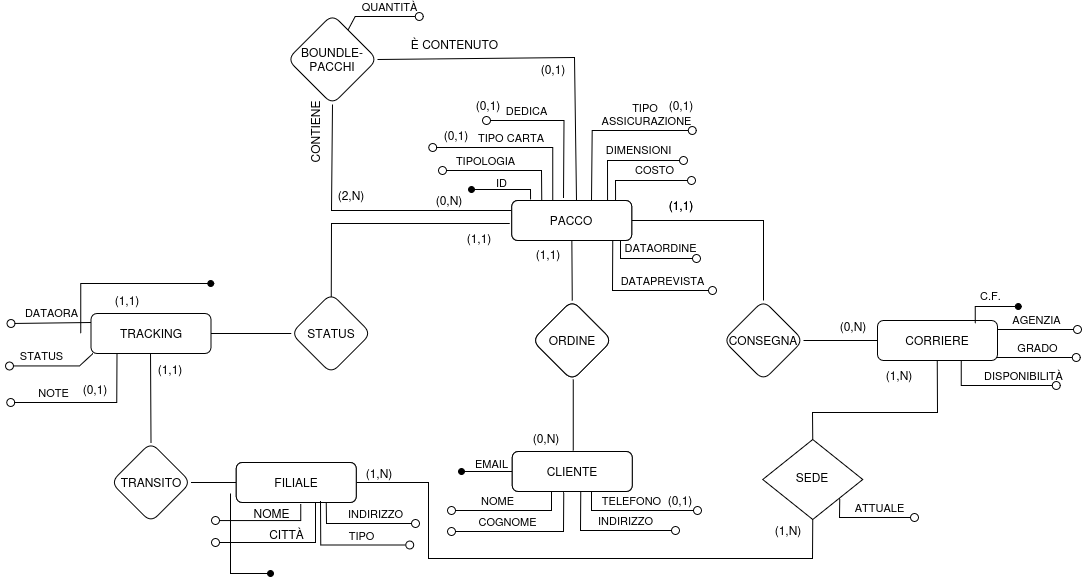
\includegraphics[width=1 \textwidth]{Resources/ML.png}
\caption{Diagramma della Base di Dati dopo l'eliminazione delle Generalizzazioni}
\label{ML}
\end{figure}

\subsection{Schema Relazionale}
Lo schema ristrutturato in Figura \ref{ML} contiene solamente costrutti mappabili in corrispettivi dello schema relazionale detto anche schema logico. Lo schema logico è rappresentato a seguire, dove l'asterisco dopo il nome degli attributi indica quelli che ammettono valori nulli.
\begin{itemize}
    \setlength{\itemindent}{+0in}
    \item \textbf{Pacco}(\underline{ID}, Tipologia, Dimensioni, Costo, DataOraOrdine, DataOraPrevista, Cliente, Corriere, TipoAssicurazione*, Dedica*, TipoCarta*)
        \begin{itemize}
            \setlength{\itemindent}{+.2in}
            \item Pacco.Cliente $\rightarrow$ Cliente.Email 
            \item Pacco.Corriere $\rightarrow$ Corriere.C.F.
        \end{itemize}
    \item \textbf{Bundle-Pacchi}(\underline{IdBundle, IdContenuto}, Quantità)
        \begin{itemize}
            \setlength{\itemindent}{+.2in}
            \item Bundle.IdBundle $\rightarrow$ Pacco.Id 
            \item Bundle.IdContenuto $\rightarrow$ Pacco.Id
        \end{itemize}
        
    \item \textbf{Corriere}(\underline{C.F.}, Agenzia, Grado, Disponibilità, Pacchi Attivi)
    \item \textbf{Filiale}(\underline{Nome, Città}, Tipo, Indirizzo)
    \item \textbf{Tracking}(\underline{IdPacco, DataOra}, Status, Note*, NomeCheckPoint,\\CittàCheckPoint)
        \begin{itemize}
                \setlength{\itemindent}{+.2in}
                \item Tracking.IdPacco $\rightarrow$ Pacco.Id
                \item Tracking.(NomeCheckPoint, CittàCheckPoint) $\rightarrow$ Filiale.(Nome, Città)
        \end{itemize}
    \item \textbf{Cliente}(\underline{Email}, Nome, Cognome, Indirizzo, Telefono*)
     \item \textbf{Sede}(\underline{Corriere, SedeNome, SedeCittà}, Attuale)
        \begin{itemize}
            \setlength{\itemindent}{+.2in}
            \item Sede.Corriere $\rightarrow$ Corriere.C.F.
            \item Sede.(SedeNome, SedeCittà) $\rightarrow$ Filiale.(Nome, Città)
        \end{itemize}
     
\end{itemize}
